\section{Programming Paradigm}
\label{programmingparadigm}
To get an understanding of the programming style and paradigm, we must consider the user group. It is essential to create a language, which is both easy to learn and still rich in features to complete its task. Many languages today are designed for a specific problem domain – an example is Lisp which is useful for symbolic data manipulation and having a complex data structure. The programming language C is good for low-level systems programming. While very low-level programming languages, like Assembly, may be challenging for a novice user, who does not have a basic understanding of Computer Science, may have a tough time to get into assembly language programming, from an experienced user. As an essential factor from this, we must dig into the target group, and find the most common programming languages to compare.  \\
\\
From the earlier analysis, the focus of this system was to create a programming system, in which an ordinary user, without any previous programming experience, can use, with a manual and learn. In this case, the focus group is very novice users, who may have touched a little, to no code in their lifetime. Looking at some of the early programming languages for this user group, we must consider some of the earlier programming languages, which has been used in educational purposes and have a low learning curve. Some of the early programming languages which have had success were Basic, which is a high-level programming language, which is a part of the programming paradigm Non-structured, and later procedural (which is structured). Another programming language, which got created for the educational purpose in 1967, named Logo. Logo is a programming language, which is in the family with Lisp, and got the programming paradigms: functional, educational, procedural and reflective.\cite{scott2000programming} \\  
\\
To bring a typical pattern in the programming languages which got mentioned in this section, all of them got a common factor, that they run on procedural paradigm, which is the opposite of the modern object-orientated paradigm, which is being used by many of the prominent languages today (Java, C\# etc.). Why is it, that object orientated paradigm is not well used for novice users, for educational purposes? - Looking at an article by Jacques Le Normand on Medium.org, Jacques reflects through this question, and the following reflections came up:\cite{tutlisp}\cite{medlisp} \\
\begin{itemize}
    \item Object orientated paradigm was not the first paradigm, and at most time is not even an appropriate paradigm for smaller tasks; however, it is one of the more prevalent paradigms in many industries today.   
    \item Object orientation thinking requires much work and can be referred to as English essays, which most students do not particularly enjoy learning to write.\cite{tutlisp}\cite{medlisp}
\end{itemize}\\
Reflecting through this, object orientated paradigms might not be a good first language, as it got a more profound learning curve than a procedural paradigm. As Jacques mentioned in his article, object orientation requires skills to understand, where procedural programming is straight forward without proper knowledge of classes and objects.


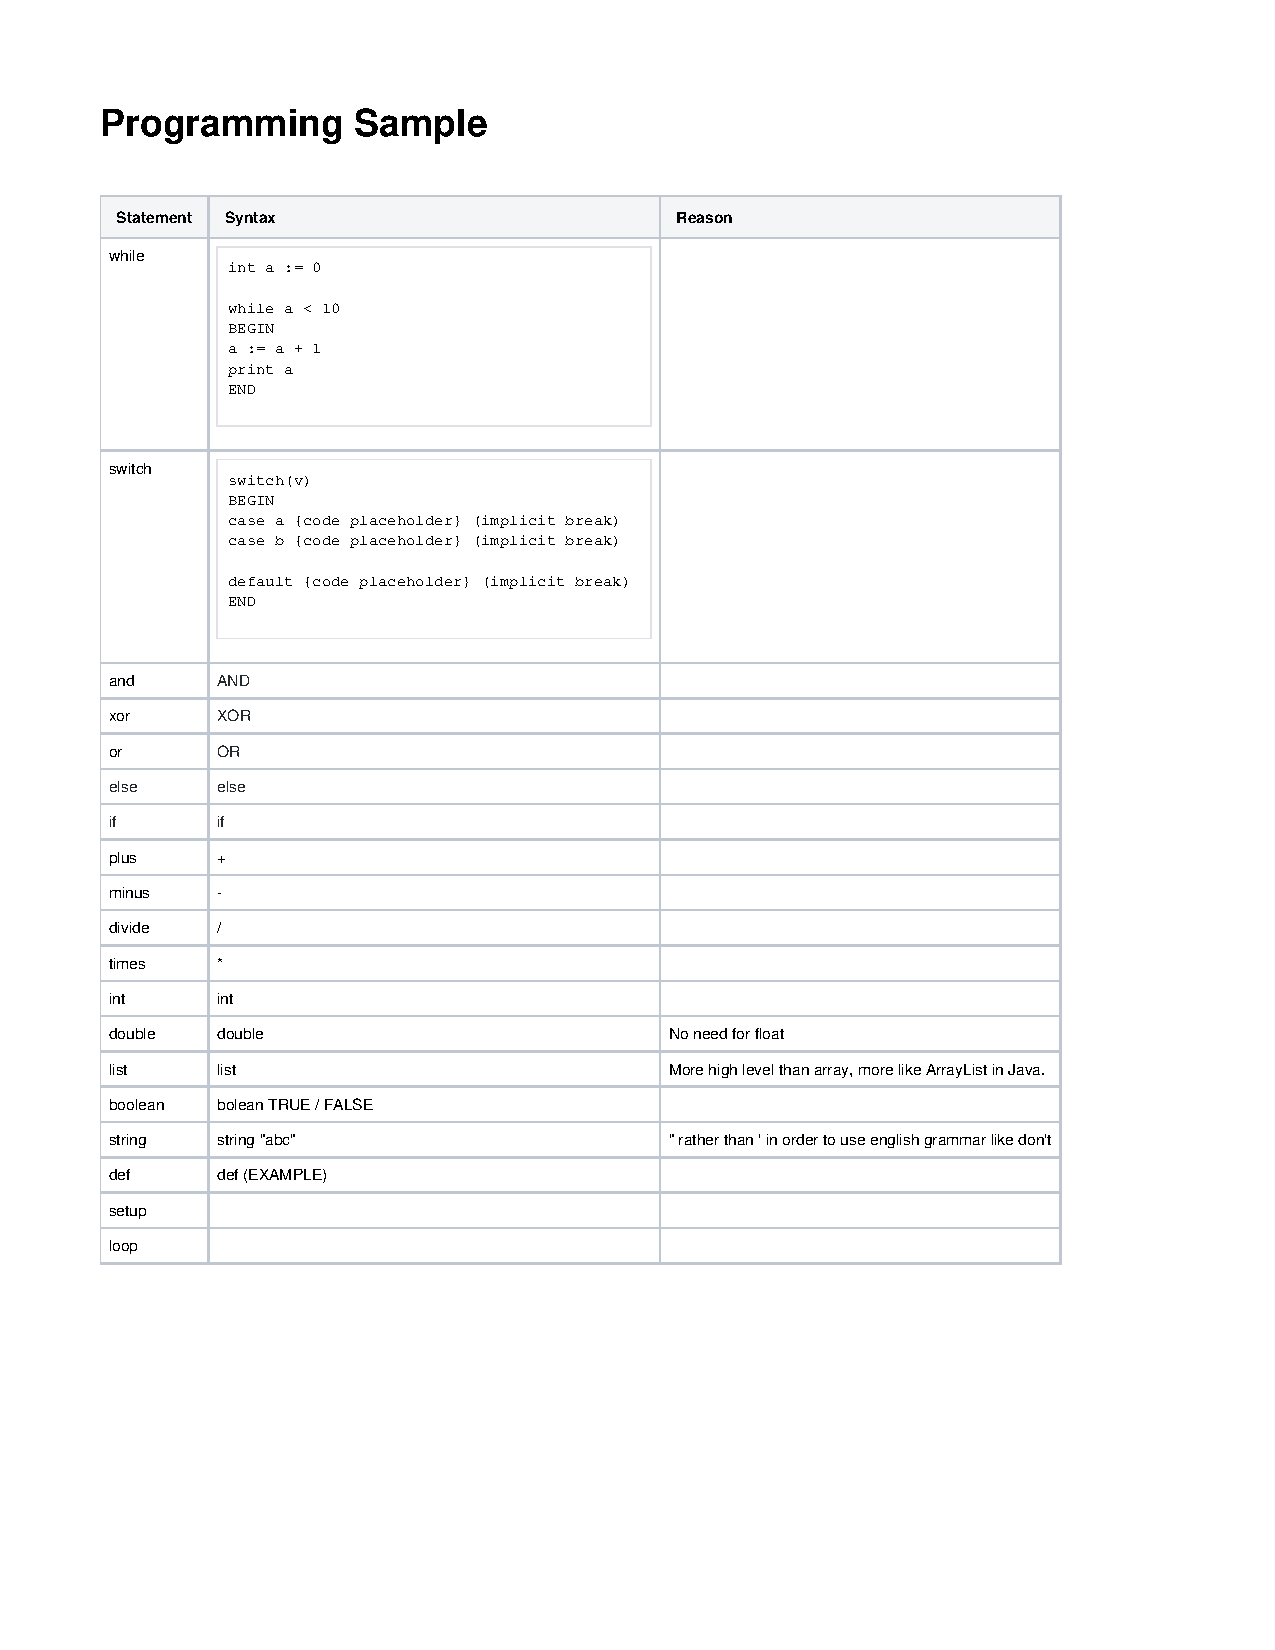
\includegraphics[scale=0.95]{sections/Analyze_phase/pdf/PL-ProgrammingSample-210219-1034-7.pdf}